\documentclass[11pt]{beamer}
\usetheme{Madrid}
\usefonttheme{serif}

\usepackage[utf8]{inputenc}       % Encoding
\usepackage[english]{babel}       % Language
\usepackage[T1]{fontenc}          % Font encoding

\usepackage{amsmath, amsfonts, amssymb} % Math packages
\usepackage{graphicx}
\usepackage{xcolor}
\usepackage{colortbl}
\usepackage{array}
\usepackage{subcaption}

\usepackage{tikz}
\usepackage{tikz-uml}
\usetikzlibrary{arrows.meta, positioning, calc}
\usepackage{blkarray}
\usepackage{pgfplots}
\pgfplotsset{compat=1.18}

%Tabular
\usepackage{tabularx}
\usepackage{multirow}
\usepackage[table]{xcolor}
\usepackage{enumitem}
\usepackage{booktabs}

% Code formatting
\usepackage{minted}
\usepackage{adjustbox}
\usepackage[ruled,vlined]{algorithm2e}
\SetKwProg{While}{while}{}{}
\SetKwProg{For}{for}{}{}
\SetKwProg{Function}{function}{}{}

% Custom math operators
\DeclareMathOperator{\sen}{sen}
\DeclareMathOperator{\tg}{tg}

% Numbered captions in figures/tables
\setbeamertemplate{caption}[numbered]

% Metadata
\author[Mathys Vinatier]{Mathys Vinatier}
\title{Optimized Kalman Filter}
\setbeamercovered{transparent}
\setbeamertemplate{navigation symbols}{}
\logo{\includegraphics[scale=.05]{../img/logoSNU.png}}
\institute[]{Seoul National University}
\date{\today}

% Bibliography
\usepackage{biblatex} 
\addbibresource{../references.bib}

%Glossary
\usepackage[acronym]{glossaries}
\makeglossaries
% glossary.tex (no preamble commands here)

\newacronym{PPO}{PPO}{Proximal Policy Optimizer}

\newacronym{ALS}{ALS}{Autocovariance Least-Squares}

\newacronym{FKF}{FKF}{Field Kalman Filter}

\newacronym{OKF}{OKF}{Optimized Kalman Filter}

\newacronym{NN}{NN}{Neural Network}

\newacronym{RNN}{RNN}{Recursive Neural Network}

\newacronym{LSTM}{LSTM}{Long Short-Term Memory}

\newacronym{MB}{MB}{Model Based}

\newacronym{KF}{KF}{Kalman Filter}

\newacronym{EKF}{EKF}{Extended Kalman Filter}

\newacronym{DD}{DD}{Data Driven}

\newacronym{KG}{KG}{Kalman Gain}

\newacronym{SS}{SS}{State Space}

\newacronym{MSE}{MSE}{Mean Square Error}

\newacronym{SPD}{SPD}{Symmetric Positive Definite}

\newacronym{WFA}{WFA}{Walk Forward Analysis}

\newacronym{TRPO}{TRPO}{Trust Region Policy Optimization}

\newacronym{LMA}{LMA}{Logarithmic Movement Average}

\newacronym{RL}{RL}{Reinforcement Learning}

\newacronym{MDP}{MDP}{Markov Decision Process}

\newacronym{API}{API}{Approximate Policy Iteration}

\newacronym{LR}{LR}{Logistic Regression}

\newglossaryentry{KalmanNet}{
    name={KalmanNet},
    description={Neural network-based model that integrates Kalman filtering techniques for improved state estimation in dynamic systems.}
}


\begin{document}

\begin{frame}
    \titlepage
\end{frame}

\begin{frame}{Deep QLearning model}
    \begin{center}
    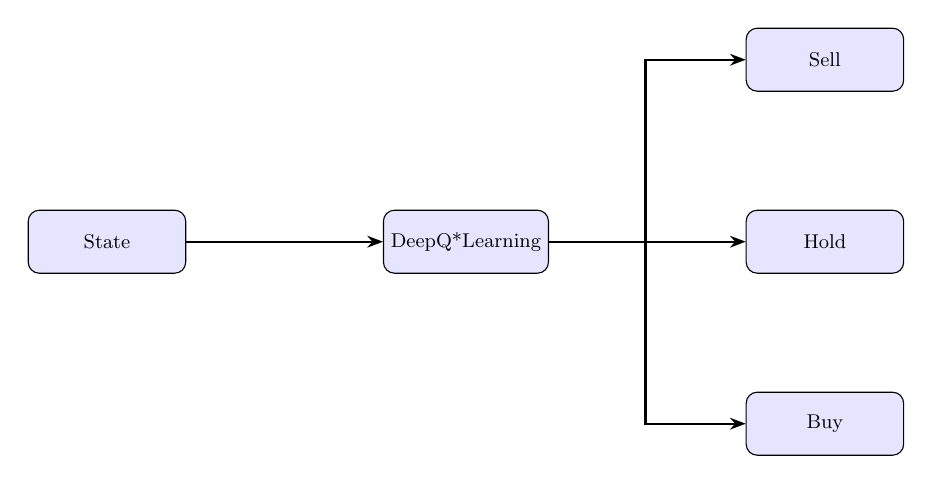
\begin{tikzpicture}[
        node distance=2.5cm,
        box/.style={
            draw,
            scale=0.8,
            rounded corners,
            minimum width=2.5cm,
            minimum height=1cm,
            align=center,
            font=\small,
            fill=blue!10
        },
        arrow/.style={
            -{Stealth[length=2mm]},
            thick
        }
    ]

    % Nodes
    \node[box] (state) {State};
    \node[box, right=of state] (dqn) {DeepQ*Learning};
    \node[box, above right=1.5cm and 2.5cm of dqn] (sell) {Sell};
    \node[box, right=of dqn] (hold) {Hold};
    \node[box, below right=1.5cm and 2.5cm of dqn] (buy) {Buy};

    % Connectors and Labels
    \coordinate (connect) at ($(dqn)!0.5!(hold)$);
    \draw[arrow] (state) -- (dqn.west);
    \draw[arrow] (connect) |- (sell);
    \draw[arrow] (connect) |- (buy);
    \draw[arrow] (dqn.east) -- (hold);

    \end{tikzpicture}
    \end{center}
\end{frame}

\begin{frame}{Deep Q-Learning Model}

    \begin{table}
        \centering
        \scalebox{0.8}{
            \begin{tabular}{ll}
                \toprule
                \textbf{Layer} & \textbf{Type} \\
                \midrule
                \texttt{nn.Linear} & Linear Layer \\
                \texttt{nn.ReLU} & Activation Function \\
                \texttt{nn.Sequential} & Container \\
                \bottomrule
            \end{tabular}
        }
        \caption{Explanation of the MLP layers}
    \end{table}

    \begin{figure}
        \centering
        \includegraphics[width=0.8\textwidth]{../img/MLP_result/QLearning_BTC-USD_2014.png}
        \caption{Performance of the Q-Learning model on a BTC-USD test set}
    \end{figure}

\end{frame} 

\begin{frame}{Deep QLearning Model}
    
    \begin{figure}[h]
        \begin{subfigure}[b]{0.49\textwidth}
            \includegraphics[width=\textwidth]{../img/MLP_result/QLearning_ATOS_2017.png}
            \caption{Performance on ATOS data from 2017.}
        \end{subfigure}
        \hfill
        \begin{subfigure}[b]{0.49\textwidth}
            \includegraphics[width=\textwidth]{../img/MLP_result/QLearning_O_2016.png}
            \caption{Performance on Realty Income (O) data from 2016.}
        \end{subfigure}
        \hfill
        \begin{subfigure}[b]{0.49\textwidth}
            \includegraphics[width=\textwidth]{../img/MLP_result/QLearning_RNO_2016.png}
            \caption{Performance on Renault (RNO) data from 2016.}
        \end{subfigure}
        \hfill
        \begin{subfigure}[b]{0.49\textwidth}
            \includegraphics[width=\textwidth]{../img/MLP_result/QLearning_TSLA_2019.png}
            \caption{Performance on Tesla (TSLA) data from 2019.}
        \end{subfigure}
    \end{figure}


\end{frame}

\begin{frame}{Deep QLearning Model}

    \begin{table}[h!]
        \centering
        \scalebox{0.8}{
        \begin{tabular}{|l l|}
            \toprule
            \textbf{Layer} & \textbf{Type} \\
            \midrule
            \texttt{DecisionTransformerGPT2Model} & Transformer Backbone \\
            \texttt{nn.Linear} (Input) & Linear Layer \\
            \texttt{nn.Linear} (Q-Head) & Linear Layer \\
            \bottomrule
        \end{tabular}}
        \caption{Explanation of the Decision Transformer layers}
    \end{table}

    \begin{figure}[h!]
        \centering
        \includegraphics[width=0.8\textwidth]{../img/GPT_transformer_results/DeepQLearning_O_2016_v2.png}
        \caption{Performance of the Deep Q-Learning Model on Realty Income (O) data from 2016.}
    \end{figure}

\end{frame}

\begin{frame}{Deep QLearning Model}

    \begin{figure}[h!]
        \centering
        \includegraphics[width=\textwidth]{../img/GPT_transformer_results/DeepQLearning_AAPL_2010.png}
        \caption{Performance of the Transofrmer Model on Apple data from 2010.}
    \end{figure}

\end{frame}

\begin{frame}{Creating Market Model}

    \centering

    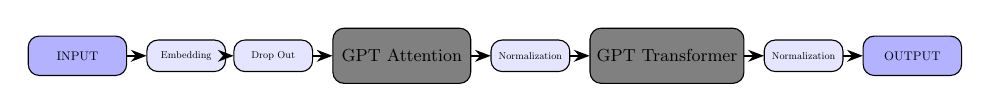
\begin{tikzpicture}[scale=0.5, transform shape,
        node distance=0.5cm,
        box/.style={draw, rounded corners, minimum width=2.5cm, minimum height=1cm, align=center, font=\small, fill=blue!10},
        arrow/.style={-{Stealth[length=2mm]}, thick}]
        \node[box, fill=blue!30] (input) {INPUT};
        \node[box, right=of input, scale=0.8] (embedding) {Embedding};
        \node[box, right=0.2cm of embedding, scale=0.8] (drop) {Drop Out};
        \node[box, right=of drop, fill=gray, scale=1.4] (attention) {GPT Attention};
        \node[box, right=of attention, scale = 0.8] (normalization1) {Normalization};
        \node[box, right=of normalization1, fill=gray, scale=1.4] (transformer) {GPT Transformer};
        \node[box, right=of transformer, scale=0.8] (normalization2) {Normalization};
        \node[box, right=of normalization2, fill=blue!30] (out) {OUTPUT};
        \draw[arrow] (input) -- (embedding);
        \draw[arrow] (embedding) -- (drop);
        \draw[arrow] (drop) -- (attention);
        \draw[arrow] (attention) -- (normalization1);
        \draw[arrow] (normalization1) -- (transformer);
        \draw[arrow] (transformer) -- (normalization2);
        \draw[arrow] (normalization2) -- (out);
    \end{tikzpicture}

    \vspace{2cm}

    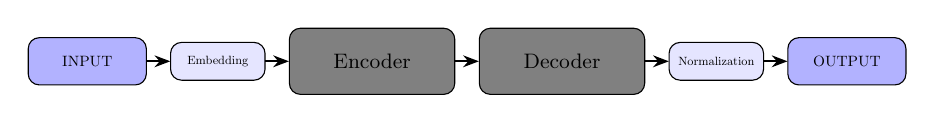
\begin{tikzpicture}[scale=0.6, transform shape,
        node distance=0.5cm,
        box/.style={draw, rounded corners, minimum width=2.5cm, minimum height=1cm, align=center, font=\small, fill=blue!10},
        arrow/.style={-{Stealth[length=2mm]}, thick}
    ]
        \node[box, fill=blue!30] (input) {INPUT};
        \node[box, right=of input, scale=0.8] (embedding) {Embedding};
        \node[box, right=of embedding, fill=gray, scale=1.4] (encoder) {Encoder};
        \node[box, right=of encoder, fill=gray, scale=1.4] (decoder) {Decoder};
        \node[box, right=of decoder, scale=0.8] (normalization) {Normalization};
        \node[box, right=of normalization, fill=blue!30] (out) {OUTPUT};
        \draw[arrow] (input) -- (embedding);
        \draw[arrow] (embedding) -- (encoder);
        \draw[arrow] (encoder) -- (decoder);
        \draw[arrow] (decoder) -- (normalization);
        \draw[arrow] (normalization) -- (out);
    \end{tikzpicture}

\end{frame}

\begin{frame}{Creating Market Model}

    \centering
    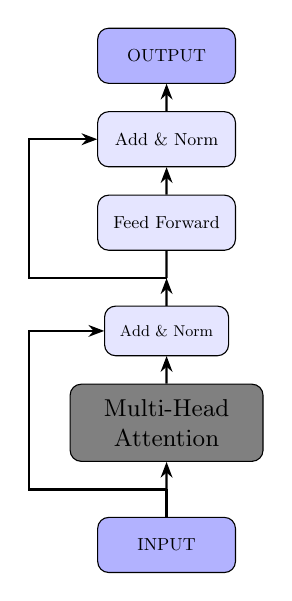
\begin{tikzpicture}[scale=0.7, transform shape,
        node distance=0.5cm,
        box/.style={draw, rounded corners, minimum width=2.5cm, minimum height=1cm, align=center, font=\small, fill=blue!10},
        arrow/.style={-{Stealth[length=2mm]}, thick},
        line/.style={thick}
    ]
        \node[box, fill=blue!30] (input) {INPUT};
        \node[coordinate, above=of input] (junction1) {} ;
        \node[box, above=of junction1,fill=gray ,scale=1.4] (mha) {Multi-Head\\ Attention};
        \node[box, above=of mha, scale=0.9] (AddNorm1) {Add \& Norm};
        \node[coordinate, above=of AddNorm1] (junction2) {} ;
        \node[box, above=of junction2] (ff) {Feed Forward} ;
        \node[box, above=of ff] (AddNorm2) {Add \& Norm} ;
        \node[box, above=of AddNorm2, fill=blue!30] (output) {OUTPUT};
        \draw[line] (input.north) -- (junction1);
        \draw[arrow] (junction1) -- (mha);
        \draw[arrow] (mha) -- (AddNorm1);
        \draw[arrow] (junction1.west) -- ++(-2.5, 0) |- (AddNorm1.west);
        \draw[arrow] (AddNorm1) -- (junction2);
        \draw[line] (junction2) -- (ff);
        \draw[arrow] (ff) -- (AddNorm2);
        \draw[arrow] (junction2.west) -- ++(-2.5, 0) |- (AddNorm2.west);
        \draw[arrow] (AddNorm2) -- (output);
    \end{tikzpicture}

\end{frame}

\begin{frame}{Creating Market Model}

    \begin{figure}[ht]
        \centering
        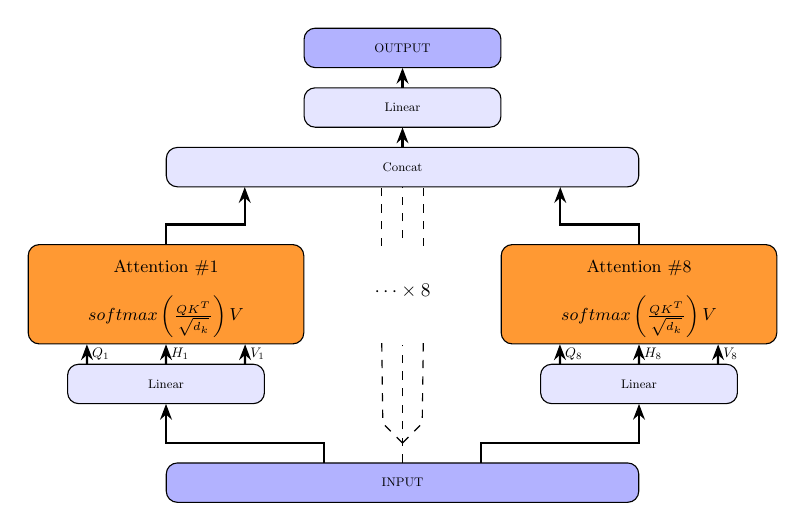
\begin{tikzpicture}[
            scale=0.5,
            transform shape,
            node distance=0.5cm,
            box/.style={
                draw,
                rounded corners,
                minimum width=5cm,
                minimum height=1cm,
                align=center,
                font=\small,
                fill=blue!10
                },
                arrow/.style={-{Stealth[length=2mm]}, thick},
                line/.style={thick}
                ]

            % Nodes
            \node[box, fill=blue!30, minimum width=12cm] (input) {INPUT};

            %Attention head #1
            \node[box, above=2cm of input.west] (linear1) {Linear};
            \node[box, above=of linear1, fill=orange!80, scale=1.4] (attention1) {\\Attention \#1\\ \\ $softmax\left( \frac{QK^T}{\sqrt{d_k}} \right)V$};

            %Dot x8
            \node[above=4cm of input, scale=1.4] (dots) {$\cdots\vspace{3mm}\times 8$};

            %Attention head #8
            \node[box, above=2cm of input.east] (linear8) {Linear};
            \node[box, above=of linear8, fill=orange!80, scale=1.4] (attention8) {\\Attention \#8\\ \\ $softmax\left( \frac{QK^T}{\sqrt{d_k}} \right)V$};

            % Output
            \node[box, above=7cm of input, minimum width=12cm] (concat) {Concat};
            \node[box, above=of concat] (linear3) {Linear};
            \node[box, above=of linear3, fill=blue!30] (output) {OUTPUT};

            % ========================================================================================

            % Connectors
            \draw[arrow]  ([xshift=-20mm]input.north)  -- ++(0, 0.5) -|  (linear1) ;
            \draw[dashed] ([yshift=+5mm]input.north) -- ++(-0.5,0.5)  --   ([xshift=-5.3mm ,yshift=-8mm]dots.south) ;
            \draw[dashed] (input.north)  --   ([yshift=-10mm]dots.south) ;
            \draw[dashed] ([yshift=+5mm]input.north) -- ++(0.5,0.5)  --   ([xshift=+5.3mm ,yshift=-8mm]dots.south) ;
            \draw[arrow]  ([xshift=20mm]input.north)  -- ++(0, 0.5) -|  (linear8) ;
        
            %Attention head #1
            \draw[arrow] ([xshift=5mm]linear1.north west)  --  ([xshift=15mm]attention1.south west) node[midway, right] {$Q_1$};
            \draw[arrow] (linear1.north)                   --  (attention1) node[midway, right] {$H_1$};
            \draw[arrow] ([xshift=-5mm]linear1.north east) --  ([xshift=-15mm]attention1.south east) node[midway, right] {$V_1$};
            \draw[arrow] (attention1.north)                -- ++(0, 0.5) -|  ([xshift=20mm]concat.south west) ;
        
            %Dot x8
            \draw[dashed] ([xshift=-5.3mm, yshift=+8mm]dots.north) -- ([xshift=-5.3mm]concat.south) ;
            \draw[dashed] ([yshift=+10mm]dots.north)  --   (concat) ;
            \draw[dashed] ([xshift=+5.3mm ,yshift=+8mm]dots.north) -- ([xshift=+5.3mm]concat.south) ;
        
            %Attention head #2
            \draw[arrow] ([xshift=5mm]linear8.north west)  --  ([xshift=15mm]attention8.south west) node[midway, right] {$Q_8$};
            \draw[arrow] (linear8.north)                   --  (attention8) node[midway, right] {$H_8$};
            \draw[arrow] ([xshift=-5mm]linear8.north east) --  ([xshift=-15mm]attention8.south east) node[midway, right] {$V_8$};
            \draw[arrow] (attention8.north)                -- ++(0, 0.5) -|  ([xshift=-20mm]concat.south east) ;


            \draw[arrow] (concat)                          --  (linear3) ;
            \draw[arrow] (linear3)                         --  (output) ;

    \end{tikzpicture}
    \caption{Multi-Head Attention stack (x8 heads)}
    \vspace{-.8cm}
    \end{figure}

\end{frame}

\begin{frame}{Creating Market Model}

    \begin{figure}[h]
    \centering
    \begin{minipage}{.45\linewidth}
        \centering
        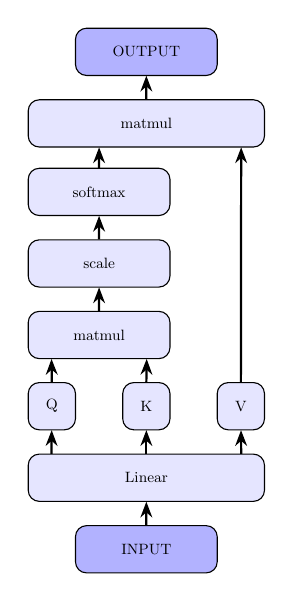
\begin{tikzpicture}[
            scale=0.6,
            transform shape,
            node distance=0.5cm,
            box/.style={
                draw,
                rounded corners,
                minimum width=3cm,
                minimum height=1cm,
                align=center,
                font=\small,
                fill=blue!10
                },
                arrow/.style={-{Stealth[length=2mm]}, thick},
                line/.style={thick}
                ]

            % Nodes
            \node[box, fill=blue!30] (input) {INPUT};
            \node[box, above=of input.north, minimum width=5cm] (linear) {Linear};
            \node[box, above=of linear.north, anchor=south west, minimum width=1cm] (q) at (linear.north west) {Q};
            \node[box, above=of linear.north, minimum width = 1cm]      (k) {K};
            \node[box, above=of linear.north, anchor=south east, minimum width=1cm] (v) at (linear.north east) {V};
            \node[box, above=of q] (matmul) at ($(q)!0.5!(k) + (0,0.5)$) {matmul};
            \node[box, above=of matmul] (scale) {scale};
            \node[box, above=of scale] (softmax) {softmax};
            \node[box, above=8cm of input, minimum width=5cm] (matmulOut) {matmul};
            \node[box, above=of matmulOut, fill=blue!30] (output) {OUTPUT};

            % Connectors
            \draw[arrow] (input.north) -- (linear);
            \draw[arrow] ([xshift=5mm]linear.north west)  -- (q);
            \draw[arrow] (linear.north) -- (k);
            \draw[arrow] ([xshift=-5mm]linear.north east) -- (v);
            \draw[arrow] (q.north)     -- ([xshift=5mm]matmul.south west);
            \draw[arrow] (k.north)     -- ([xshift=-5mm]matmul.south east);
            \draw[arrow] (matmul)      -- (scale);
            \draw[arrow] (scale)       -- (softmax);
            \draw[arrow] (softmax)     -- ([xshift=-10mm]matmulOut.south);
            \draw[arrow] (v)           -- ([xshift=-5mm]matmulOut.south east);
            \draw[arrow] (matmulOut)   -- (output);

        \end{tikzpicture}
        \caption{Attention stack}
    \end{minipage}\hspace{.5cm}
    \begin{minipage}{.45\linewidth}
        \centering
        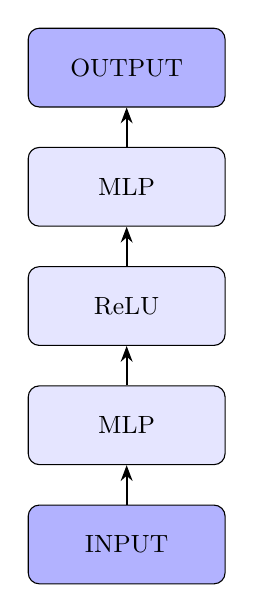
\begin{tikzpicture}[
            scale=1,
            transform shape,
            node distance=0.5cm,
            box/.style={
                draw,
                rounded corners,
                minimum width=2.5cm,
                minimum height=1cm,
                align=center,
                font=\small,
                fill=blue!10
                },
                arrow/.style={-{Stealth[length=2mm]}, thick},
                line/.style={thick}
                ]

                % Nodes
                \node[box, fill=blue!30] (input) {INPUT};
                \node[box, above=of input] (mlp1) {MLP};
                \node[box, above=of mlp1] (relu) {ReLU};
            \node[box, above=of relu] (mlp2) {MLP};
            \node[box, above=of mlp2, fill=blue!30] (output) {OUTPUT};

            % Connectors
            \draw[arrow] (input.north) -- (mlp1);
            \draw[arrow] (mlp1)        -- (relu);
            \draw[arrow] (relu)        -- (mlp2);
            \draw[arrow] (mlp2)        -- (output);

        \end{tikzpicture}
        \caption{Feed-Forward stack}
    \end{minipage}
    \end{figure}

\end{frame}

\begin{frame}{Adding commission}
    %
    \begin{figure}[h!]
        \centering
        \includegraphics[width=0.8\textwidth]{../img/expriment_on_commission/DeepQLearning_TSLA_2019_commission.png}
        \caption{Performance of the Deep Q-Learning Model with commission on Tesla data from 2019.}
    \end{figure}

\end{frame}

\begin{frame}{Reworking the Reward}

    \begin{figure}[h!]
        \centering
        \includegraphics[width=\textwidth]{../img/reward_portfolio.png}
        \caption{Reward based on portfolio}
    \end{figure}

\end{frame}

\begin{frame}{Reworking the Reward}

    \begin{figure}[h!]
        \centering
        \includegraphics[width=\textwidth]{../img/reward_portfolio_difference.png}
        \caption{Reward based on portfolio differences}
    \end{figure}

\end{frame}

\begin{frame}{Reworking the Reward}

    \begin{figure}[h!]
        \centering
        \includegraphics[width=\textwidth]{../img/reward_portfolio_times_derivate.png}
        \caption{Reward based on portfolio times the velocity}
    \end{figure}

\end{frame}

\begin{frame}{Reworking the Reward}

    \begin{figure}[h!]
        \centering
        \includegraphics[width=\textwidth]{../img/reward_portfolio_times_derivate_additive.png}
        \caption{Reward based on added portfolios times the velocity}
    \end{figure}

\end{frame}

\begin{frame}{Reworking the Reward}

    \begin{figure}[h!]
        \centering
        \includegraphics[width=\textwidth]{../img/reward_portfolio_times_derivate_additive_log.png}
        \caption{Reward based on added portfolios times the velocity with logarithmic function}
    \end{figure}

\end{frame}

\begin{frame}
    \centering
    \vspace{2cm}
    {\LARGE Thank You}
\end{frame}

\end{document}
